\documentclass[12pt]{scrartcl}
\usepackage[sexy]{james}
\usepackage[noend]{algpseudocode}
\setlength {\marginparwidth}{2cm}
\usepackage{answers}
\usepackage{array}
\usepackage{tikz}
\newenvironment{allintypewriter}{\ttfamily}{\par}
\usepackage{listings}
\usepackage{xcolor}
\usetikzlibrary{arrows.meta}
\usepackage{color}
\usepackage{mathtools}
\newcommand{\U}{\mathcal{U}}
\newcommand{\E}{\mathbb{E}}
\usetikzlibrary{arrows}
\Newassociation{hint}{hintitem}{all-hints}
\renewcommand{\solutionextension}{out}
\renewenvironment{hintitem}[1]{\item[\bfseries #1.]}{}
\renewcommand{\O}{\mathcal{O}}
\declaretheorem[style=thmbluebox,name={Chinese Remainder Theorem}]{CRT}
\renewcommand{\theCRT}{\Alph{CRT}}
\setlength\parindent{0pt}
\usepackage{sansmath}
\usepackage{pgfplots}

\usetikzlibrary{automata}
\usetikzlibrary{positioning}  %                 ...positioning nodes
\usetikzlibrary{arrows}       %                 ...customizing arrows
\newcommand{\eqdef}{=\vcentcolon}
\newcommand{\tr}{{\rm tr\ }}
\newcommand{\im}{{\rm Im\ }}
\newcommand{\spann}{{\rm span\ }}
\newcommand{\Col}{{\rm Col\ }}
\newcommand{\Row}{{\rm Row\ }}
\newcommand{\dint}{\displaystyle\int}
\newcommand{\dt}{\ {\rm d }t}
\newcommand{\PP}{\mathbb{P}}
\newcommand{\horizontal}{\par\noindent\rule{\textwidth}{0.4pt}}
\usepackage[top=3cm,left=3cm,right=3cm,bottom=3cm]{geometry}
\newcommand{\mref}[3][red]{\hypersetup{linkcolor=#1}\cref{#2}{#3}\hypersetup{linkcolor=blue}}%<<<changed

\tikzset{node distance=4.5cm, % Minimum distance between two nodes. Change if necessary.
         every state/.style={ % Sets the properties for each state
           semithick,
           fill=cyan!40},
         initial text={},     % No label on start arrow
         double distance=4pt, % Adjust appearance of accept states
         every edge/.style={  % Sets the properties for each transition
         draw,
           ->,>=stealth',     % Makes edges directed with bold arrowheads
           auto,
           semithick}}


% Start of document.
\newcommand{\sep}{\hspace*{.5em}}

\pgfplotsset{compat=1.18}
\begin{document}
\title{AMSC460: Homework 1}
\author{James Zhang\thanks{Email: \mailto{jzhang72@terpmail.umd.edu}}}
\date{\today}

\definecolor{dkgreen}{rgb}{0,0.6,0}
\definecolor{gray}{rgb}{0.5,0.5,0.5}
\definecolor{mauve}{rgb}{0.58,0,0.82}

\lstset{frame=tb,
  language=Java,
  aboveskip=3mm,
  belowskip=3mm,
  showstringspaces=false,
  columns=flexible,
  basicstyle={\small\ttfamily},
  numbers=left,
  numberstyle=\tiny\color{gray},
  keywordstyle=\color{blue},
  commentstyle=\color{dkgreen},
  stringstyle=\color{mauve},
  breaklines=true,
  breakatwhitespace=true,
  tabsize=3
}

\maketitle

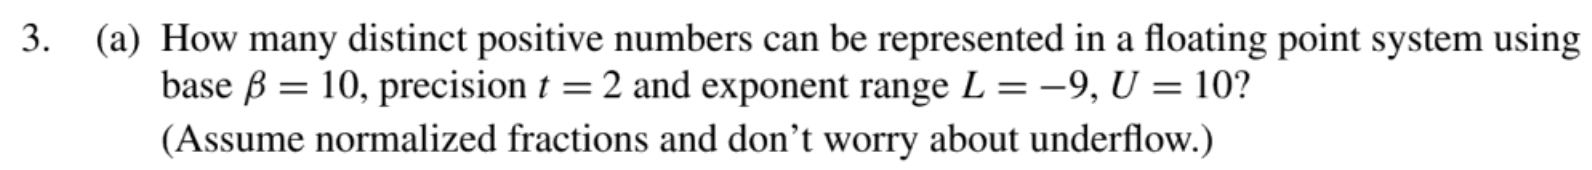
\includegraphics[width=14cm]{3a.png}

\begin{proof}[Solution]
  In general, a floating point number can be expressed in the representation 
  \[fl(x) = \pm \left( \frac{\overset{\sim}{d}_0}{\beta^0} + \frac{\overset{\sim}{d}_1}{\beta^1} + \cdots 
  + \frac{\overset{\sim}{d}_{t-1}}{\beta^{t-1}}\right) \times \beta^e\]
  The problem statement specifies that we are looking for positive integers, $t = 2$, $\beta = 10$, and 
  $e$ is bounded by $-9$ and $10$. Applying this information, we now have the more specific representation 
  \[fl(x) = + \left( \overset{\sim}{d}_0 + \frac{\overset{\sim}{d}_1}{10}\right) \times 10^e\]
  Since we assume normalized fractions, $\overset{\sim}{d}_0 \neq 0$, so it can attain the digits $1-9$, or $9$ possibilties. 
  $\overset{\sim}{d}_1$ can be any digit, so $10$ possibilities. Finally, $e$ can be any number from $-9$ to $10$, so $20$ possibilities. 
  Multiplying these together yields 
  \[9 \times 10 \times 20 = 1800 \text{ distinct positive integers }\]
\end{proof}

\newpage

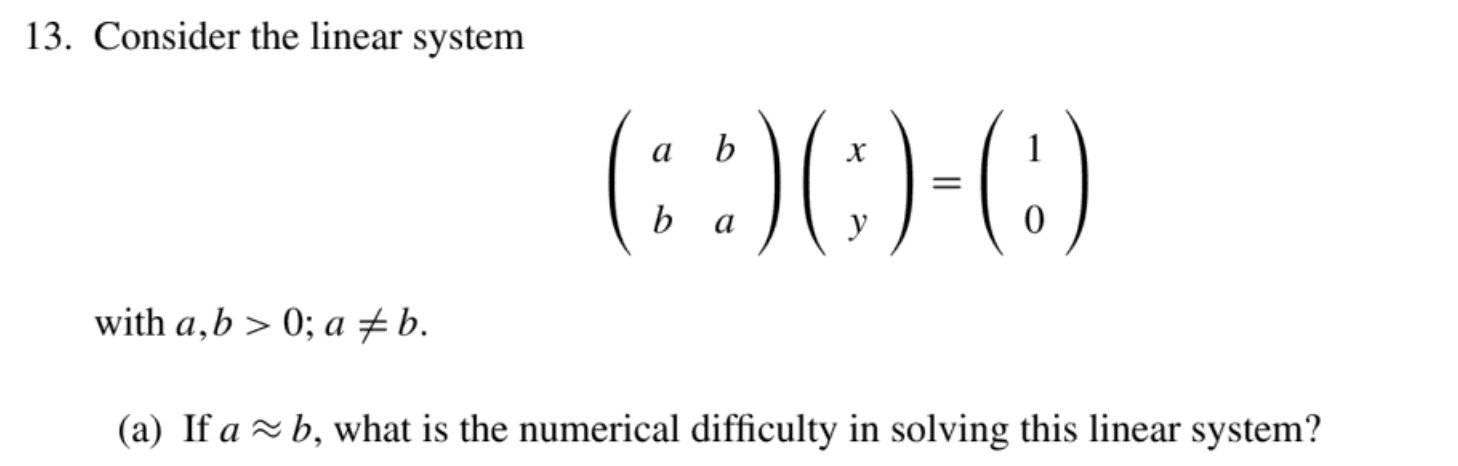
\includegraphics[width=14cm]{13a.png}

\begin{proof}[Solution]
  To solve this system, if the square matrix is invertble, we would invert the matrix 
  and solve for the vector $\begin{pmatrix}
    x & y
  \end{pmatrix}^T$. By the Invertible Matrix Theorem, one of the conditioning for checking if a matrix is invertible is if 
  its determinant is nonzero. Note that the determinant of the square matrix is 
  \[\det\begin{pmatrix}
    a & b\\
    b & a
  \end{pmatrix} = a^2 - b^2 = (a-b)(a+b)\]
  If $a \approx b$, and specifically if we take the limit $a-b\to 0$, 
  \[\lim_{a-b\to 0} \det\begin{pmatrix}
    a & b\\ b & a
  \end{pmatrix} = 0\]
  because the $a-b$ approaches $0$. Therefore, the matrix is almost singular and so the system is very ill-condtioned, 
  meaning the system output is sensititve to small changes in coefficients and that small errors in arithmetic will get quickly propagated 
  throughout the calculations. 
\end{proof}

\newpage 


\includegraphics[width=14cm]{1a.png}

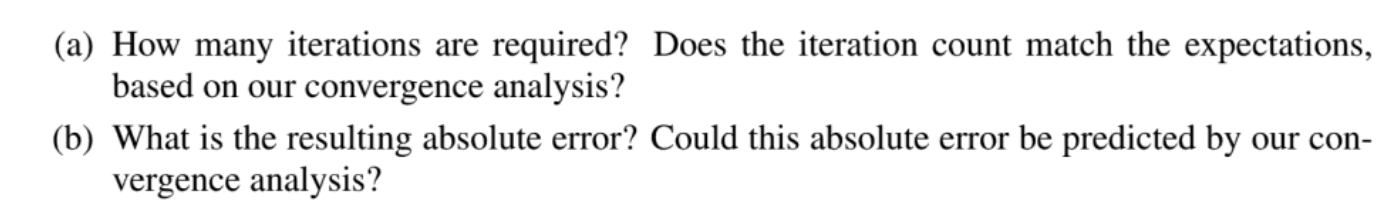
\includegraphics[width=14cm]{1b.png}

\begin{proof}[Solution]
  \hfill

  \begin{enumerate}[(a)]
    \item Let us apply the Bisection Method 
    
    \begin{lstlisting}[language=Matlab]
function [root, iter] = bisection_sqrt()
  % Define the function
  f = @(x) sqrt(x) - 1.1;
  
  % Set the tolerance and initial interval [a, b]
  atol = 1e-8;
  a = 0;
  b = 2; % Initial guess for the root search range
  
  % Check if the interval is valid
  if f(a) * f(b) > 0
      error('f(a) and f(b) must have opposite signs');
  end
  
  iter = 0; % Counter for number of iterations
  
  % Bisection method loop
  while (b - a) / 2 > atol
      iter = iter + 1;
      c = (a + b) / 2; % Midpoint of interval
      if f(c) == 0
          break; % We've found the exact root
      elseif f(a) * f(c) < 0
          b = c; % Root lies in the left subinterval
      else
          a = c; % Root lies in the right subinterval
      end
  end

root = (a + b) / 2; % Approximate root

% Display the result
fprintf('Root found: %.10f\n', root);
fprintf('Number of iterations: %d\n', iter);
fprintf('Error: %.10f\n', root - 1.21)
end
    \end{lstlisting}

    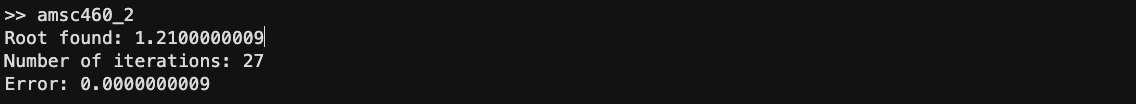
\includegraphics[width=13cm]{root_found.png}

    We can compute the expected number of iterations as 
    \[\text{Expected Iterations} = \text{ceil}\left( \frac{\log(b-a) - \log(2 * \text{atol})}{\log 2}\right) = \text{ceil}(26.57) = 27\]
    and this matches with our true number of iterations, $27$. 

  \item The resulting absolute error is $0.0000000009 = 9 \times 10^{-10} < \text{atol} = 1 \times 10^{-8}$. Using a convergence analysis, we know that 
    the error is always less than half the length of the current interval. In words, after the first interval, 
    we know that our error will be less than $\frac{1}{2} = 2^{-1}$. After the second iteration, the error will be less than $\frac{1}{4} = 2^{-2}$. To generalize this, 
    after the $i$-th iteration, our error will be less than $2^{-i}$. Since we computed that the bisection method will have 
    an expected number of iterations equal to $28$, we can say that our error is upper bounded by 
    \[\text{Predicted error} = 2^{-28} = \frac{1}{2^{28}} \approx 0.00000000372529 \approx 3.72529 \times 10^{-9}\]
    and we can correctly observe that
    \begin{align*}
      \text{True error} \leq \text{Predicted Error} \leq \text{atol}\\
      9 \times 10^{-10} \leq 3.72529 \times 10^{-9} \leq 1 \times 10^{-8}
    \end{align*}

\end{enumerate}

\end{proof}

\newpage 

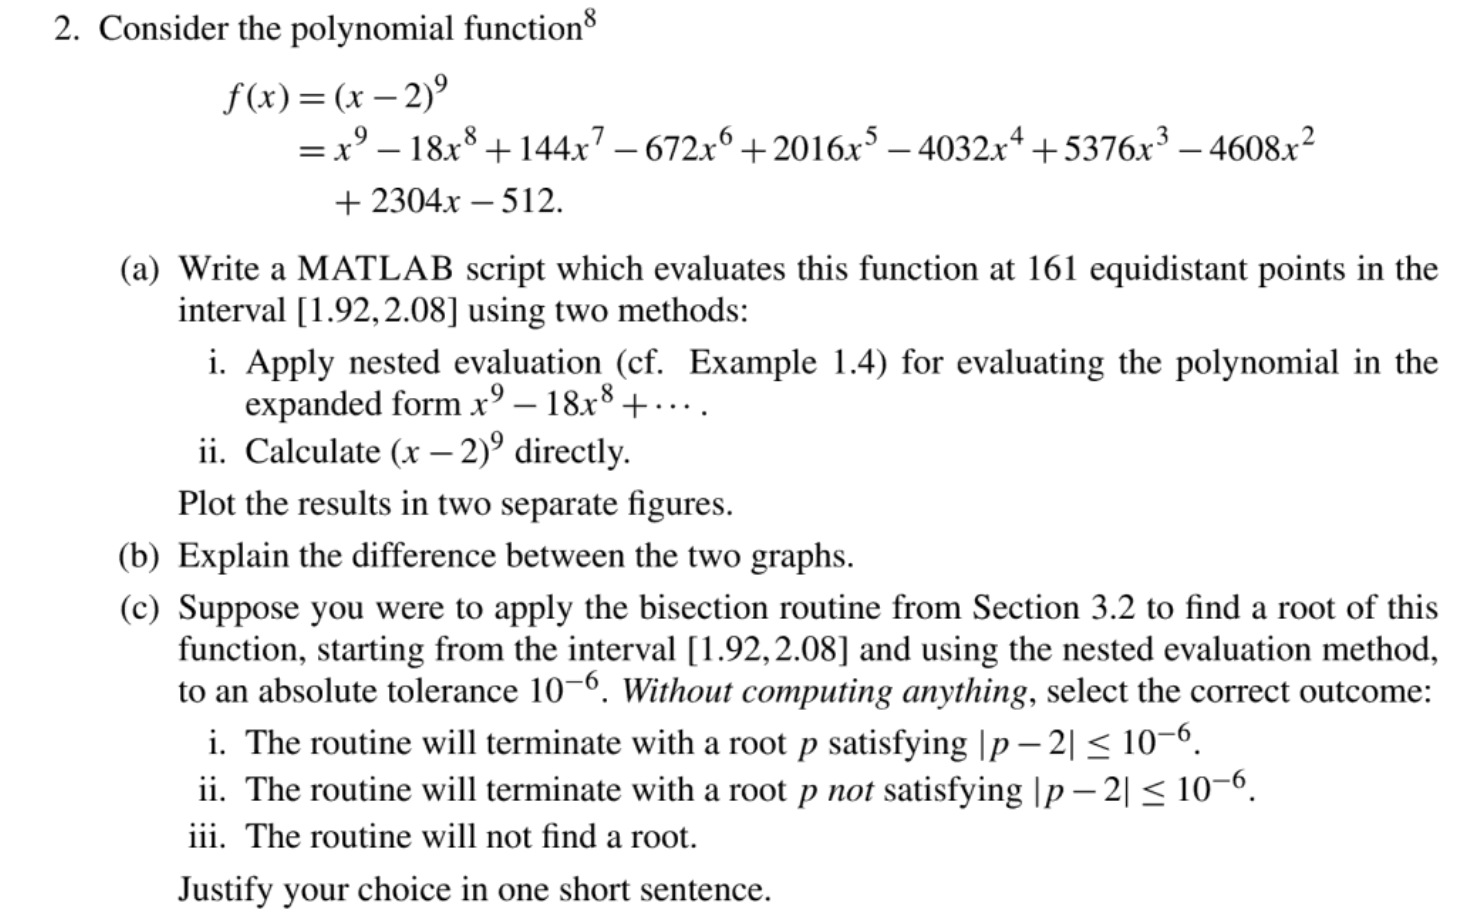
\includegraphics[width=14cm]{2.png}

\begin{proof}[Solution]
\hfill

\begin{enumerate}[(a)]
  \item Below is my Matlab code
  
  \begin{lstlisting}[language=Matlab]
% Define the polynomial coefficients
c = [1, -18, 144, -672, 2016, -4032, 5376, -4608, 2304, -512];
% Nested evaluation function (Horner's method)
function y = nested_eval(x, c)
    n = length(c) - 1;
    y = c(1);
    for j = 2:n+1
        y = y.*x + c(j);
    end
end
% Direct calculation function
f2 = @(x) (x - 2).^9;
% Generate 161 equidistant points in [1.92, 2.08]
x = linspace(1.92, 2.08, 161);
% Evaluate the function using both methods
y1 = nested_eval(x, c);
y2 = f2(x);
% Plot the results
figure(1)
plot(x, y1)
title('Method 1: Nested Evaluation (Horner''s Method)')
xlabel('x')
ylabel('f(x)')
figure(2)
plot(x, y2)
title('Method 2: Direct Calculation')
xlabel('x')
ylabel('f(x)')
  \end{lstlisting}

  \begin{center}
    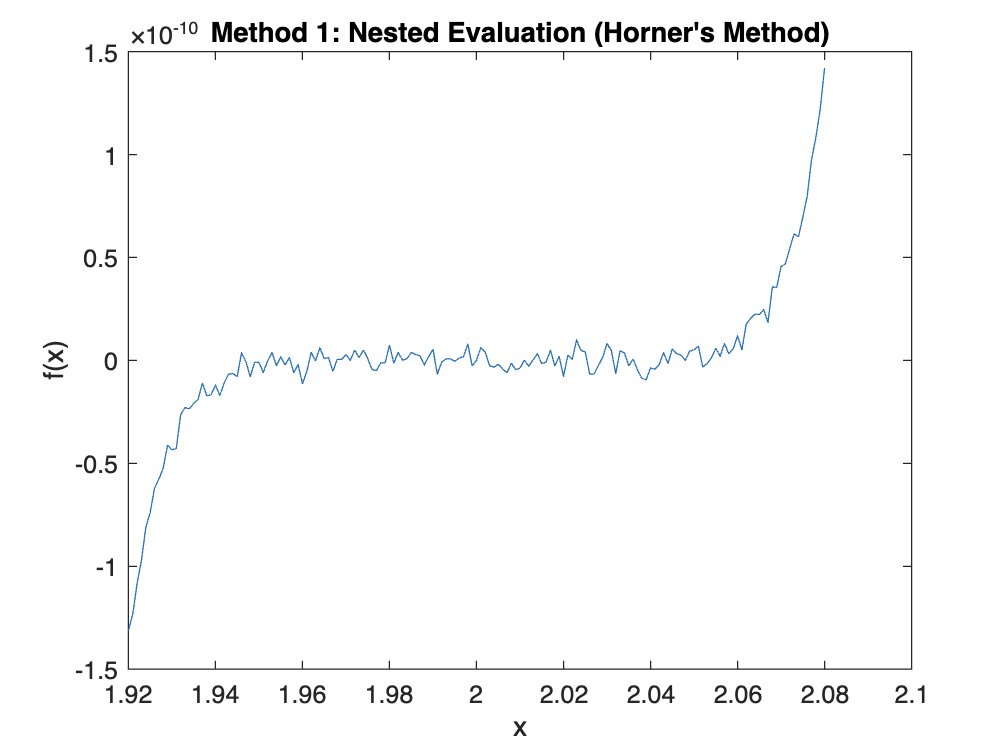
\includegraphics[width=6.75cm]{method1.png}
    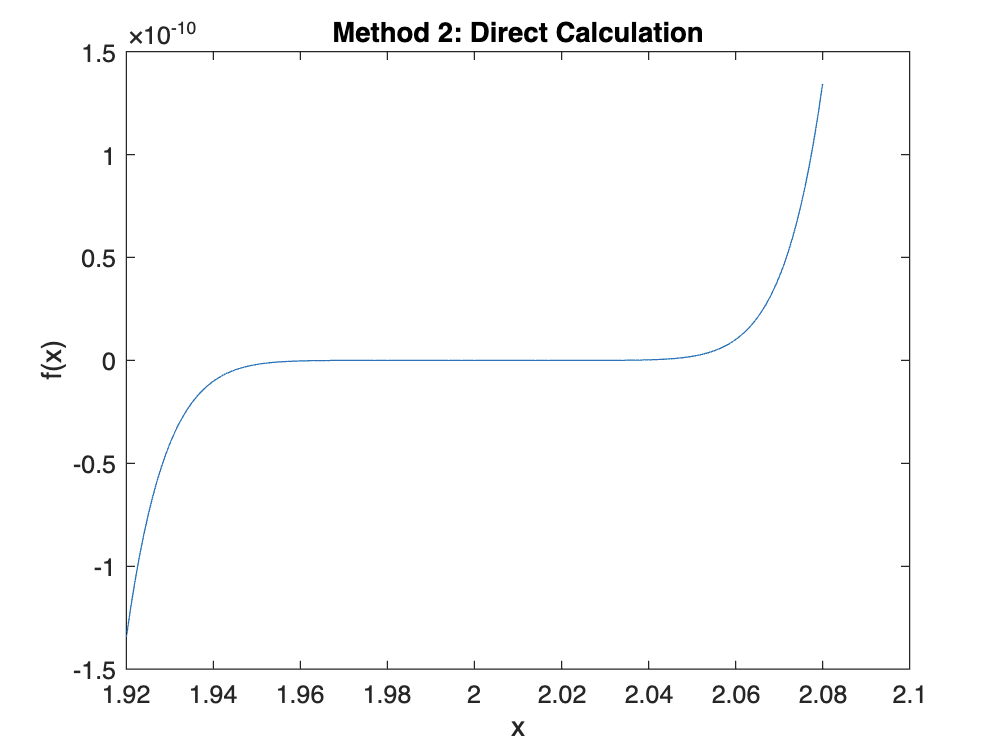
\includegraphics[width=6.75cm]{method2.png}
  \end{center}

\item The graph of Method 2 is far more smooth and symmetric about $x=2$ then Method 1, which shows 
many more oscillations due to the numerical instability of the method. Method 1 involves multiple arithmetic operations 
with large and small numbers. Each operation introduces small rounding errors due to the 
finite precision of floating-point arithmetic in computers. Furthermore, in the expanded form, errors 
from calculations propagate and amplify through subsequent operations. In direct calculation, the output 
is more numerically stable because it avoids the intermediate large numbers and repeated operations that 
cause issues in Method 1. 

\item In the case where we use the textbook code for Bisection Method, I would select choice $ii$ because in that code, 
there is no check for if we have found the exact root ($f(p) == 0$), so it will continuously make the interval smaller, and since Nested Evaluation is numerically unstable here, it is likely that Bisection Method 
converges to a root that does not satisfy the provided atol = $1 \times 10^{-6}$. However, in a more efficient implementation of Bisection Method, I propose 
the following alternative answer of Choice $i$. 

Choice $i$: despite the Nested Evaluation method being more numerically unstable than Direct Evaluation, let us actually think about if we were to 
proceed using the Bisection Method. In the first iteration $a = 1.92, b = 2.08 \implies p = 2$ (which is the exact root of $f(x) = (x-2)^9$)
and since $2$ is an integer and the terms in the polynomial will not result in integer overflow, there will be no floating point or rounding errors, and the Bisection Method will find the exact 
root $p = 2$ in the first iteration, satisfying the tolerance condition perfectly. 
\end{enumerate}

\end{proof}

\end{document}

